\chapter{Results}\label{chap:results}
\begin{jointwork}
    Sections~\ref{sec:results:measurement}--\ref{sec:results:exclusion} are adapted from Ref.\,\cite{Walter2024_LFthermal}.
\end{jointwork}

The scanning strategy developed in Chapter~\ref{chap:experiment} is applied here to the proof-of-concept methanol search. This chapter presents the measurement, data-analysis pipeline, candidate evaluation, and resulting exclusion limits.


\section{The methanol measurement}\label{sec:results:measurement}

The scanning framework developed in Sections~\ref{sec:experiment:single}--\ref{sec:experiment:optimization} was applied in a proof-of-concept ALP search using the CASPEr-Gradient-LF apparatus with a thermally polarized methanol sample. This section describes the measurement procedure and parameters. In the following, $g_\mathrm{ap}$ denotes the ALP-proton gradient coupling constant, i.e.\ $g_\mathrm{aNN}$ evaluated for proton spins.

\subsection{Measurement parameters}

The search covered a \SI{240}{\Hz} band centered at \SI{1.348570}{\MHz}, corresponding to proton Larmor frequencies driven by a bias field $|\mathbf{B}_0| \approx \SI{31.67}{\milli\tesla}$. This maps to ALP masses in the range $5.576741$--$5.577733\,\si{\neV}/c^2$. The frequency step size was \SI{6}{\Hz}, approximately half the NMR linewidth, so that the resonant windows of adjacent steps overlap. Three sequential scans over the same range were performed. The most sensitive scan was treated as the primary scan and the other two (scans A and B) as consistency checks.

The ALP coherence time at the search frequency is $\tau_a \approx \SI{0.35}{\s}$, obtained from Equation~\eqref{eq:taua}. The measured relaxation times are $T_2^* = \SI{24.2\pm4}{\ms}$ and $T_2 = \SI{0.72(5)}{\s}$. Since $T_2^* \ll \tau_a \lesssim T_2$, the measurement falls in regime~(2) of Table~\ref{tab:summary_of_regimes}. The spectral factor is approximately $u \approx T_2^*/\tau_a \approx \SI{7}{\%}$.

\subsection{Step sequence}

At each frequency step the following actions were performed in order:
\begin{enumerate}[label=\arabic*.]
    \item Pulsed-NMR measurement (a $\pi/2$ pulse followed by free-induction decay) to determine the Larmor frequency, linewidth $\Delta\nu$ (and hence $T_2^* = 1/(\pi\Delta\nu)$), and NMR signal power. A Lorentzian fit to the resulting PSD peak extracts these parameters and calibrates the sensitivity at each step.
    \item Carr-Purcell-Meiboom-Gill (CPMG) \cite{CPMG} pulse sequence prior to the first scan step to determine $T_2$ from the exponential decay of spin-echo amplitudes.
    \item \SI{5}{\s} dwell time to allow ring-down noise to decay and the magnetization to return close to its equilibrium value along $\mathbf{B}_0$.
    \item \SI{100}{\s} data acquisition without any pulses, recording the SQUID feedback voltage $V_\mathrm{f}$ at \SI{13.4}{\kHz} sampling rate. This window corresponds to approximately 280 ALP coherence times and is the ALP-search channel.
    \item Frequency step: the Larmor frequency is increased by \SI{\approx6}{\Hz} by ramping the Helmholtz coils or the superconducting magnet.
    \item Another \SI{5}{\s} dwell time after the field ramp before repeating.
\end{enumerate}
The PSDs were recorded after demodulation of $V_\mathrm{f}$ by the lock-in amplifier; its reference frequency was detuned by \SI{820}{\Hz} from the Larmor frequency so that the NMR signal appears at a non-zero difference frequency, making it easily distinguishable from noise. Example PSD spectra and NMR characterization plots are shown in Figure~\ref{fig:measurements}.

\begin{figure*}[htb]
    \centering
    
\includegraphics[width=\linewidth]{works/LF-thermal/figures/measurements.png}
    \caption{
    \textbf{(a)} PSD after a $\pi/2$ pulse. The NMR peak is fitted with a Lorentzian (red line); the center is at \SI{1348449.21(5)}{\Hz} with a FWHM of \SI{14.79(1)}{\Hz}.
    \textbf{(b)} CPMG spin-echo amplitudes (blue dots) and exponential fit (red), giving $T_2 = \SI{0.72(5)}{\s}$.
    \textbf{(c)} PSD of a \SI{100}{\s} ALP-search step. The gray analysis window (\SI{8}{\kHz} wide) excludes filter artifacts near the band edges; the green resonant window ($\pm5$ NMR linewidths $= \pm\SI{70}{\Hz}$) is where ALP signal candidates are sought.
    \textbf{(d)} Histogram of normalized power excess (NPE) derived from (c), with the rescan threshold $\Theta_\mathrm{RE}$ (red line) at the \SI{95}{\%} confidence level for a $5\,\sigma$ ALP detection.
    Reproduced from Ref.\,\cite{Walter2024_LFthermal}.}
    \label{fig:measurements}
\end{figure*}

Due to Earth's rotation, the component of the ALP-field gradient perpendicular to $\mathbf{B}_0$ varies over the course of the measurement. The resulting daily modulation of the signal amplitude is predictable and was tracked over the approximately six-hour duration of the scans.


\section{Data analysis}\label{sec:results:analysis}

Each \SI{100}{\s} time series is converted to a PSD and processed through three successive steps.

\subsection{Spike suppression}

A narrow Savitzky-Golay (SG) filter with a window half-width equal to half the expected ALP linewidth at the scanned frequency is applied to the PSD. The residual between the raw PSD and the filter output is fitted with a $\chi^2$ distribution with two degrees of freedom. Bins that deviate from the filter response by more than the fitted threshold, together with their four nearest neighbors, are replaced by the local filter average. This step suppresses narrow EMI spikes while preserving potential ALP signals. In the primary scan, only \SI{0.002}{\%} of bins were modified in this way.

\subsection{Baseline removal}

A reduced chi-square test on the spike-corrected spectrum reveals a non-flat baseline. A second, broad SG filter with a window of 200 ALP linewidths is applied to estimate this baseline. The spike-corrected spectrum is then normalized by subtracting and dividing by this baseline, producing a spectrum with a flat expected noise floor.

\subsection{Matched filtering and NPE}

A matched filter using the expected ALP signal lineshape $\lambda_\perp(\nu,\nu_a)$---the normalized spectral lineshape of the ALP-field gradient component perpendicular to $\mathbf{B}_0$, as given in Ref.\,\cite{Gramolin2022Feb_SpectralSignatures}---is convolved with the normalized PSD. The result, normalized by its standard deviation, is the normalized power excess (NPE). The matched-filter step size is half the ALP linewidth.

\subsection{Hypothesis test and rescan threshold}

Frequency bins where the NPE exceeds the rescan threshold $\Theta_\mathrm{RE}$ are flagged as outliers. The threshold was determined via Monte Carlo simulations of the NPE distribution under the null hypothesis that a $5\,\sigma$ ALP signal is present, yielding $\Theta_\mathrm{RE} = 3.43$ at the \SI{95}{\%} confidence level (corresponding to a $p$-value of $0.001$).

The overall analysis efficiency, accounting for the effect of baseline removal on signal recovery, was determined from simulations to be $\eta_\mathrm{rec} = \SI{88.2\pm4.6}{\%}$. This efficiency is applied when converting NPE values to coupling-constant limits.


\section{Exclusion results}\label{sec:results:exclusion}

\subsection{Candidates and consistency checks}

Table~\ref{tab:candidates} lists the outlier counts and ALP signal candidates from all three scans. The total number of outliers in each scan exceeds the expectation for white noise, owing to non-white-noise structures that are neither narrow nor broad enough to be removed by the SG filters. By comparing the resonant window (within $\pm5$ NMR linewidths of the Larmor frequency) with off-resonance background, and by cross-checking the primary scan against scans A and B, these noise-induced outliers can be identified.

\begin{table}[htb]
    \centering
    \caption{Results of the three ALP scans. $N_\mathrm{full}$: total NPE bins. $X_\mathrm{full}$: outliers above rescan threshold. $\langle X_\mathrm{full}\rangle$: expected value assuming white noise. $N_\mathrm{res}$: bins in resonant windows. $X_\mathrm{res}$: ALP signal candidates. $\langle X_\mathrm{res}\rangle$: expected value. $X'_\mathrm{res}$: candidates after merging those within one ALP linewidth. $X''_\mathrm{res}$: candidates in this scan also appearing in the primary scan within four ALP linewidths. Parenthetical fractions give the fraction of $N_\mathrm{full}$.}
    \label{tab:candidates}
    \begin{tabular}{lccc}
        \hline\hline
        & Primary scan & Scan A & Scan B \\
        \hline
        $N_\mathrm{full}$ & 481\,680 & 481\,680 & 481\,680 \\
        $X_\mathrm{full}$ & 6393 (\SI{1.32}{\%}) & 5760 (\SI{1.20}{\%}) & 6202 (\SI{1.29}{\%}) \\
        $\langle X_\mathrm{full}\rangle$ & 145 (\SI{0.03}{\%}) & 145 (\SI{0.03}{\%}) & 145 (\SI{0.03}{\%}) \\
        \hline
        $N_\mathrm{res}$ & 8430 & 8430 & 8430 \\
        $X_\mathrm{res}$ & 5 & 7 & 3 \\
        $\langle X_\mathrm{res}\rangle$ & 3 & 3 & 3 \\
        $X'_\mathrm{res}$ & 5 & 5 & 3 \\
        $X''_\mathrm{res}$ & --- & 0 & 0 \\
        $\langle X''_\mathrm{res}\rangle$ & --- & 0 & 0 \\
        \hline\hline
    \end{tabular}
\end{table}

No candidate from the primary scan was found in either of the consistency-check scans within four ALP linewidths. The search therefore yields no statistically significant evidence for ALP dark matter at the detection sensitivity.

\subsection{Coupling-constant limit}


\begin{equation}
    |g_\mathrm{aNN}| \leq \sqrt{\frac{e_5}{\eta_\mathrm{rec}\,P_{\perp,1}}}
    \,,\label{eq:limcouple}
\end{equation}

In the absence of a detection, an upper limit on the ALP-proton gradient coupling is obtained from
\begin{equation}
    |g_\mathrm{ap,\,lim}| = \sqrt{\frac{e_5}{\eta_\mathrm{rec}\,P_{\perp,1}}}
    \,,\label{eq:limcouple}
\end{equation}
where $e_5$ is the signal power corresponding to the $5\,\sigma$ NPE threshold, $P_{\perp,1}$ is the reference signal power for $|g_\mathrm{ap}|=\SI{1}{\GeV^{-1}}$, and $\eta_\mathrm{rec}$ is the analysis efficiency defined above. The resulting exclusion limits are plotted in Figure~\ref{fig:ALPlimits}.

\begin{figure}[htb]
    \centering
    \includegraphics[width=\linewidth]{works/LF-thermal/figures/ALPlimits.png}
    \caption{ALP gradient-proton coupling excluded at \SI{95}{\%} confidence level by the three sequential scans. Each data point represents the sensitivity for one scan step. The variation in sensitivity between scans reflects the daily modulation of the ALP wind direction relative to the bias field. Reproduced from Ref.\,\cite{Walter2024_LFthermal}.}
    \label{fig:ALPlimits}
\end{figure}

The measurement sets the limit $|g_\mathrm{ap}| \lesssim \SI{3e-2}{\GeV^{-1}}$ over the scanned ALP mass range $5.576741$--$5.577733\,\si{\neV}/c^2$. This is the first dedicated laboratory search in this mass range. The sensitivity is dominated by the small thermal polarization of the methanol sample; hyperpolarized samples are expected to improve it by several orders of magnitude.


\section{Earth-bound ALP measurement}\label{sec:earthhalomeas}

% In this data taking, the bias field was ramped to ?? therefore the Larmor frequency of the sample was tuned to ??, corresponding to an ALP mass of \SI{}{\neV/c^2}. 
% The measurement lasted for ?? hours in total. In this section, the measurement procedure and results are presented. 

\subsection{Procedure and parameters}

A data taking with thermally polarized methanol took place at Dec 14, 2022. 
The measurement scanned 
\begin{equation}
    \SI{1.348585}{\MHz} \pm \SI{24}{\Hz} \nonumber
\end{equation}
by sweeping the magnitude of the bias field $|\mathbf{B}_0| \approx \SI{31.67403}{\milli\tesla}$.
This corresponds to an ALP mass range of 
\begin{equation}
    \SI{5.577299}{\neV/c^2} \pm \SI{50}{\femto\electronvolt/c^2}\,. \nonumber
\end{equation}
The scanning took 8 steps. 
In each scan step, the following actions were performed in order:
\begin{enumerate}[label=\arabic*.]
    \item Set sweep coil current. 
    \item 1-Pulse measurement (a $\pi/2$ pulse followed by free decay signal) to determine the Larmor frequency, linewidth $\Delta\nu$ (and hence $T_2^* = 1/(\pi\Delta\nu)$), and NMR signal power. 
    A Lorentzian fit to the resulting PSD peak extracts these parameters and calibrates the sensitivity at each step.
    \item Carr-Purcell-Meiboom-Gill (CPMG) \cite{CPMG} pulse sequence prior to the first scan step to determine $T_2$ from the exponential decay of spin-echo amplitudes.
    \item A 1-hour ALP measurement without any pulses. 
    \item 1-Pulse measurement like step 2. 
    \item CPMG measurement like step 3.    
\end{enumerate} 
Delays ($\gg T_1$) were inserted between pulsed-NMR measurements to allow the magnetization to return close to its equilibrium value along $\mathbf{B}_0$. 
A schematic of the measurement procedure is shown in Figure~\ref{fig:earthhalomeas_procedure}. 
Note that the 1-hour ALP measurement duration is much longer than the 100-second duration used in the data taking described in Section~\ref{sec:results:measurement}. The long measurement duration results in a much narrower PSD bin width, which is beneficial for the sensitivity to ALP signals with long coherence time, such as the Earth-bound ALP halo. 
\begin{figure}[htb]
    \centering
    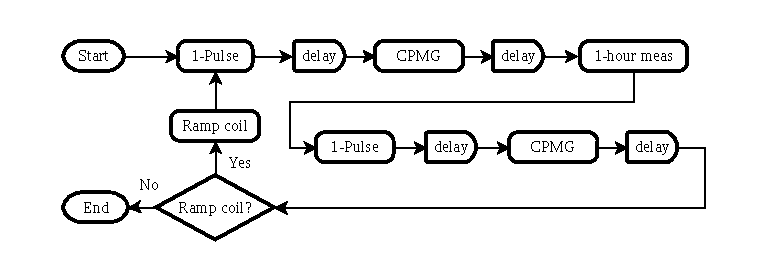
\includegraphics[width=0.99\linewidth]{figures/20221214_meas_diagram_v0.2.drawio.pdf}
    \caption{Schematic of the Earth-bound ALP measurement procedure.}
    \label{fig:earthhalomeas_procedure}
\end{figure}
A summary of the measurement parameters is given in Table~\ref{tab:earthmeas_params}. 
Long measurement durations make this measurement sensitive to the long-coherence-time ALP fields. 
Therefore, this measurement is chosen to demonstrate the sensitivity of the CASPEr-Gradient-LF apparatus to the Earth-bound ALP halo model. 

\begin{table}[htb]
    \centering
    \caption{Technical parameters of the Earth-bound ALP measurement (December 14, 2022). Here SNR indicates the signal-to-noise ratio of the free decay signal after a $\pi/2$ pulse.}
    \label{tab:earthmeas_params}
    \begin{tabular}{lc}
        \toprule
        Parameter & Name or value \\
        \hline
        Sample & thermally polarized methanol \\
        Number of scan steps & 8 \\
        Sweep coil current increment & \SI{0.8}{\mA} \\
        Frequency increment per step & \SI{6}{\Hz} \\
        Frequency scan range & $\SI{1.348585}{\MHz} \pm \SI{24}{\Hz}$ \\
        NMR linewidth (FWHM) in one step & $\approx\SI{10}{\Hz}$ \\
        $T_2$ relaxation time & $\approx\SI{1}{\s}$ \\
        Signal-to-noise ratio (SNR) & $\approx 120$ \\
        Axion measurement duration per step & \SI{1}{\hour} \\
        \bottomrule
    \end{tabular}
\end{table}



\subsection{Expected signal and sensitivity}

% periodic modulation of the signal amplitude due to the daily rotation of the Earth is expected.
Due to the daily rotation of the Earth, the component of the ALP-field gradient perpendicular to $\mathbf{B}_0$ varies over the course of the measurement. 
Using the ALP signal model established in Chapter~\ref{sec:theory:earthALP}, the expected signal amplitude can be calculated. 
In Figure~\ref{fig:earthhalomeas_signal}, the evolution of the expected Rabi frequency of the pseudomagnetic field is plotted (assuming all ALPs are at $2p$ state). 
Since the Rabi frequency $\Omega_a \approx 2 \pi \times \SI{1}{\mHz}$, the tipping angle of the magnetization can be estimated as $\theta \approx \Omega_a T_2 \approx 0.002\, \pi$. 

\begin{figure}[htb]
    \centering
    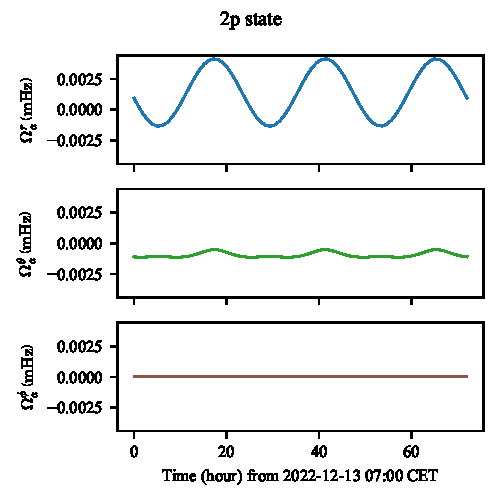
\includegraphics[width=0.95\linewidth]{figures/earth_halo_expected_rabi_evolution.pdf}
    \caption{Expected evolution of the ALP-induced Rabi frequency (pseudomagnetic field) over one sidereal day for the Earth-bound ALP halo model. The amplitude modulation is driven by the daily rotation of the laboratory frame relative to the ALP-field gradient; the plotted curve shows the combined effect of the geometry of $\mathbf{B}_0$ and the predicted halo profile. }
    \label{fig:earthhalomeas_signal}
\end{figure}
